\section{Технический проект}
\subsection{Общая характеристика организации решения задачи}

Необходимо спроектировать и разработать приложение, которое обеспечит функционирование СКУД на круизном лайнере AIDABlu.

Приложение представляет собой панель управления, представляющую набор взаимосвязанных таблиц в базе данных системы. Панель содержит текстовую и графическую информацию (TreeView).

Приложение является десктопным, т.е. располагается и запускается внутри лишь одной операционной системы. Каждое окно приложения (за исключением главного) – это панель управления для конкретной таблицы базы данных. Приложение написано на языке Python v3.10. Управление таблицами БД реализовано с помощью библиотеки sqlite3 и SQL -- языка структурированных запросов к базе данных.

\subsection{Общие сведения о программно-информационной системе}

Полное наименование системы: Программное обеспечение для системы контроля и управления доступом на круизном судне.

Краткое обозначение системы: \textquotedbl СКУД на круизном лайнере \textquotedbl.

Описание системы: \textquotedbl СКУД на круизном лайнере \textquotedbl предназначена для корпораций, организующих круизные путешествия, предоставляя им платформу для удобного контроля и управления данными всей бизнес-системы круизного лайнера на время поездки. Система создана для обеспечения комфортной и безопасной поездки каждого пассажира и функционирования даже в форс-мажорных ситуациях.

Условия эксплуатации: \textquotedbl СКУД на круизном лайнере \textquotedbl предназначена для использования как в нормальных, так и в чрезвычайных условиях работы.

Архитектура системы: Программное обеспечение основано на десктопной архитектуре, используя современные технологии разработки, включая TKinter для Front-End части и sqlite3 для реализации запросов к БД в Back-End. Система использует базу данных SQLite.

Технологии и инструменты: В разработке использовались tkinter, sqlite3, asyncio, time

\subsection{Обоснование выбора технологии проектирования}

\subsubsection{Описание используемых технологий и языков программирования}

В процессе разработки приложения используются программные средства и языки программирования. Каждое программное средство и каждый язык программирования применяется для круга задач, при решении которых они необходимы.

\subsubsection {tkinter}
Выбор tkinter для Front-End обосновывается его простотой и кроссплатформенной поддержкой, а также минимальными требованиями к интерфейсу в пользу быстродействия. 

Пакет tkinter («интерфейс Tk») - это интерфейс Python для создания GUI. Tkinter доступен на большинстве платформ Unix, включая macOS, а также на системах Windows.

Tkinter входит в состав большинства инсталляций Python, что делает его легкодоступным для разработчиков, которые хотят создавать приложения с графическим интерфейсом, не требуя дополнительных инсталляций или библиотек.

\subsubsection {SQLite}
Выбор SQLite в качестве системы управления базами данных также обосновывается его удобством как на этапе проектирования, так и на этапе реализации.

SQLite - это библиотека на языке C, которая предоставляет легкую дисковую базу данных, не требующую отдельного серверного процесса и позволяющую обращаться к базе данных с помощью нестандартного варианта языка запросов SQL. Некоторые приложения могут использовать SQLite для внутреннего хранения данных. Также можно создать прототип приложения с использованием SQLite, а затем перенести код на более крупную базу данных, такую как PostgreSQL или Oracle.

\subsubsection {asyncio и time}
Модули asyncio и time были использованы для актуализации работы системы в реальном времени и многопоточном режиме.


\subsubsection{Язык структурированных запросов к базе данных SQL}
SQL - это стандартизированный язык программирования, который используется для управления реляционными базами данных и выполнения различных операций над данными в них. 

SQL используется для следующего:
\begin{itemize}
	\item изменение структуры таблиц и индексов базы данных;
	\item добавление, обновление и удаление строк данных;
	\item извлечение подмножеств информации из реляционных систем управления базами данных (РСУБД).
\end{itemize}


\subsubsection{Язык программирования Python}

\paragraph{Достоинства языка Python}
Python - очень продуктивный язык. Благодаря простоте Python разработчики могут сосредоточиться на решении проблемы. Написание кода экономит время и освобождает его для более ёмкой работы с другими составляющими проекта.

Python поставляется под лицензией OSI с открытым исходным кодом. Это делает его свободным для использования и распространения. Можно загружать исходный код, изменять его и даже распространять свою версию Python. Это полезно для организаций, которые хотят изменить некоторые специфические функции и использовать свою версию для разработки.

Стандартная библиотека Python огромна, в ней можно найти практически все функции, необходимые для решения любой задачи. Таким образом, не придется зависеть от внешних библиотек.

Во многих языках, таких как C/C++, для запуска программы на разных платформах необходимо изменять код. С Python дело обстоит иначе. Вы пишете один раз и запускаете программу в любом месте.

\paragraph{Недостатки языка Python}

Язык программирования Python использует большой объем памяти. Это может быть недостатком при создании приложений, когда мы предпочитаем оптимизацию памяти.

Python обычно используется для программирования на стороне сервера. Мы не видим Python на стороне клиента или в мобильных приложениях.

Python - динамически типизированный язык, поэтому тип данных переменной может измениться в любой момент. Переменная, содержащая целое число, в будущем может стать строкой, что может привести к ошибкам времени выполнения.

\subsection{Проектирование пользовательского интерфейса}
На основании требований к пользовательскому интерфейсу, представленных в пункте 2.3 технического задания, был разработан графический интерфейс десктопного приложения с применением python tkinter, ttk и SQLite. Этот процесс подчеркивает важность интуитивно понятного и эффективного взаимодействия с пользователем. Разработанный интерфейс ориентирован на обеспечение легкости в использовании и интуитивного понимания функционала приложения, предоставляя пользователю простое и эффективное взаимодействие с приложением.

1. Навигация по таблицам: Реализация функции навигации на основе полей psr\underline{ }btn, psr\underline{ }ua\underline{ }btn, drs\underline{ }btn, rms\underline{ }btn, pns\underline{ }btn;

2. Отдельные интерфейсы для каждой таблицы с полями: диверсификация интерфейсов происходит на основе метода show\underline{ }table;

3. Отображение текущей таблицы в реальном времени: актуальность этого графического элемента (дерева) поддерживается за счёт методов TreeRefresh и TreeCreate;

4. Возможность так или иначе воздействовать на внесённые данные базы внутри приложения: Добавление, изменение или удаление элементов реализованы в методах add\underline{ }element, update\underline{ }element и delete\underline{ }element соответственно, внутри которых формирование строк запросов к БД реализовано с помощью класса Utils.

5. Понятная навигация и лёгкий поиск среди элементов конкретной таблицы: Пользователь может переходить по элементам последовательно (метод MoveTo класса main), или же использовать отдельное текстовое поле для метода search\underline{ }element, перейдя сразу к искомому элементу таблицы.

6. Отображение локального времени: Учитывая специфику проекта -- систему для круизного лайнера, учтём, что часовой пояс может измениться во время путешествия. На уровне python и SQL была установлена привязка к локальному времени (localtime), а функционал часов запущен в асинхронном потоке во избежание ошибок и помех работы основной системы.

\subsection{Диаграмма размещения}

Диаграмма размещения, отображаемая на рисунке \ref{fig:commonscheme4}, является фундаментальным инструментом для иллюстрации взаимосвязей между программными и аппаратными компонентами системы. Этот элемент визуализации служит для акцентирования значимости стратегического планирования
в процессе разработки распределенных систем. Детальное и глубокое понимание этих взаимосвязей критически важно для успешного создания и функционирования распределенных информационных систем.

Каждый компонент системы, будь то программный или аппаратный, играет важную роль в обеспечении её общей эффективности и надежности.
Подход, основанный на стратегическом планировании, способствует оптимизации этих взаимодействий и повышает вероятность успешной реализации и эксплуатации системы в целом.


\begin{figure}
	\centering
	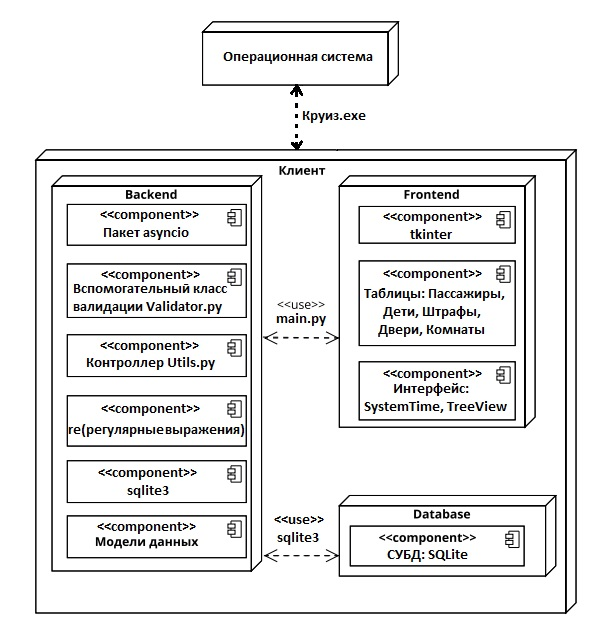
\includegraphics[width=1\linewidth]{images/CommonScheme4}
	\caption{Диаграмма размещения}
	\label{fig:commonscheme4}
\end{figure}


Она является хорошим средством для показа маршрутов перемещения объектов и компонентов в распределенной системе.

\subsection{Описание архитектуры приложения}

Архитектура приложения, реализованная в рамках текущего исследования, базируется на модели FUN (Flat hierarchy, Utility styles,  Name-spaced components). 
Этот паттерн был избран благодаря его способности делать код удобно создаваемым и поддерживаемым.

За каждой буквой названия стоит определенный принцип:

\begin{itemize}
	\item F, плоская иерархия полей;
	\item U, служебные классы: поощряется создание служебных классов для решения типовых задач контроля, напр. запроса к базе данных.
	\item N, компоненты с неймспейсами: Рекомендуется добавлять отдельные пространства для задания правил конкретных элементов. Такой подход позволит глобализации правил и простого внедрения новых, если потребуется.
\end{itemize}

Такой подход накладывает достаточно мало требований по структуре кода и проекта, он лишь устанавливает предпочтительную форму записи организации функционала и способ его использования в тестировании. Но в небольших проектах этих правил может быть вполне достаточно для создания качественного кода.